%%%%%%%%%%%%%%%%%%%%%%%%%%%%%%%%%%%%%%%%%%%%%%%%%%%%%%%%%%%%%%%%%%%%%%%%%%%%%%%%%%%%%%%
\section{Diode Clipper Circuit}
\label{subsec:diode_clipper_intro}
%%%%%%%%%%%%%%%%%%%%%%%%%%%%%%%%%%%%%%%%%%%%%%%%%%%%%%%%%%%%%%%%%%%%%%%%%%%%%%%%%%%%%%%
\begin{figure}
  \centering
  %%%%%%%%%%%%%%%%%%%%%%%%%%%%%%%%%%%%%%%%%%%%%%%%%%%%%%%%%%%%%%%%%%%%%%%%%%%%%%%%%%%%%%%
\section{Diode Clipper Circuit}
\label{subsec:diode_clipper_intro}
%%%%%%%%%%%%%%%%%%%%%%%%%%%%%%%%%%%%%%%%%%%%%%%%%%%%%%%%%%%%%%%%%%%%%%%%%%%%%%%%%%%%%%%
\begin{figure}
  \centering
  %%%%%%%%%%%%%%%%%%%%%%%%%%%%%%%%%%%%%%%%%%%%%%%%%%%%%%%%%%%%%%%%%%%%%%%%%%%%%%%%%%%%%%%
\section{Diode Clipper Circuit}
\label{subsec:diode_clipper_intro}
%%%%%%%%%%%%%%%%%%%%%%%%%%%%%%%%%%%%%%%%%%%%%%%%%%%%%%%%%%%%%%%%%%%%%%%%%%%%%%%%%%%%%%%
\begin{figure}
  \centering
  %%%%%%%%%%%%%%%%%%%%%%%%%%%%%%%%%%%%%%%%%%%%%%%%%%%%%%%%%%%%%%%%%%%%%%%%%%%%%%%%%%%%%%%
\section{Diode Clipper Circuit}
\label{subsec:diode_clipper_intro}
%%%%%%%%%%%%%%%%%%%%%%%%%%%%%%%%%%%%%%%%%%%%%%%%%%%%%%%%%%%%%%%%%%%%%%%%%%%%%%%%%%%%%%%
\begin{figure}
  \centering
  \input{figures/tikz/diode_clipper.tex}
  \caption{Diode clipper circuit.}
  \label{fig:diode_clipper_circuit}
\end{figure}

The first-order diode clipper is a circuit frequently used to achieve signal distortion, e.g., in guitar amplifiers. Its schematic is shown in \Figure{fig:diode_clipper_circuit}. It can be regarded as consisting of two parts: an RC lowpass filter and a diode limiter.

Voltages and currents in this section are dependent on time, i.e., $V = V(t), I= I(t)$. For readability, this dependence is not stated explicitly in the equations.

%%%%%%%%%%%%%%%%%%%%%%%%%%%%%%%%%%%%%%%%%%%%%%%%%%%%%%%%%%%%%%%%%%%%%%%%%%%%%%%%%%%%%%%
\subsection{RC Lowpass Filter}
%%%%%%%%%%%%%%%%%%%%%%%%%%%%%%%%%%%%%%%%%%%%%%%%%%%%%%%%%%%%%%%%%%%%%%%%%%%%%%%%%%%%%%%

\begin{figure}
  \centering
  \input{figures/tikz/rc_lowpass.tex}
  \caption{RC lowpass filter.}
  \label{fig:rc_lowpass}
\end{figure}

The first part of the diode clipper circuit is an RC lowpass filter. An RC lowpass filter is shown in \Figure{fig:rc_lowpass}. Given that the input voltage $V_\text{in}$ is a sine wave at frequency $f$, the input-output voltage relation is governed by the following equation
\begin{equation}
  V_\text{out} = \frac{X_C}{\sqrt{R^2 + X_C^2}} V_\text{in},
  \label{eq:rc_circuit}
\end{equation}
where $V_\text{out}$ is the output voltage, $X_C=\frac{1}{2\pi f C}$ is the capacitive reactance of the capacitor in the circuit, $C$ is its capacitance, and $R$ is the resistor's resistance.

The capacitor impedes low frequencies more; the lower the frequency, the higher the capacitive reactance. More capacitive reactance means larger voltage drop on the capacitor. Thus, assuming a constant magnitude across all frequencies of the input voltage, the output voltage is higher for low frequencies. Therefore, the circuit behaves like a lowpass filter.

Considering an arbitrary input waveform, we may derive a differential equation that describes the circuit \cite{Horowitz2015}. The current $I$ through the capacitor is proportional to the rate of change of the voltage across it

\begin{equation}
  I = C \frac{\mathrm{d}V_\text{out}}{\mathrm{d} t}.
  \label{eq:current_through_capacitor}
\end{equation}

The current flowing through the resistor can be calculated using the Ohm's law as a ratio of the voltage drop across the resistor to its resistance

\begin{equation}
  I = \frac{V_\text{in} - V_\text{out}}{R}.
  \label{eq:current_through_resistor}
\end{equation}

Because the same current flows through the resistor and the capacitor we can equate the right-hand sides of \Equation{eq:current_through_capacitor} and \Equation{eq:current_through_resistor}. After dividing by $C$, we obtain the final form of the \ac{ODE} describing the RC circuit

\begin{equation}
  \frac{\mathrm{d}V_\text{out}}{\mathrm{d} t} = \frac{V_\text{in} - V_\text{out}}{RC}.
\end{equation}



%%%%%%%%%%%%%%%%%%%%%%%%%%%%%%%%%%%%%%%%%%%%%%%%%%%%%%%%%%%%%%%%%%%%%%%%%%%%%%%%%%%%%%%
\subsection{Diode Limiter}
%%%%%%%%%%%%%%%%%%%%%%%%%%%%%%%%%%%%%%%%%%%%%%%%%%%%%%%%%%%%%%%%%%%%%%%%%%%%%%%%%%%%%%%
\begin{figure}
  \centering
  \input{figures/tikz/diode_limiter.tex}
  \caption{Diode limiter circuit.}
  \label{fig:diode_limiter}
\end{figure}

The second part of the diode clipper is the diode limiter also called a \emph{diode clamp} \cite{Malvino2016}. Its circuit is shown in \Figure{fig:diode_limiter}. It consists of two inversely polarized diodes and a resistor. This circuit could be further divided into a \emph{positive clipper} (by removing the diode on the left) and a \emph{negative clipper} (by removing the diode on the right). These names refer to which part of the input \ac{AC} signal (the positive or the negative) is removed at the output.

If the diodes were ideal, i.e., they would behave as an open for voltages across smaller than 0 and as a short for voltages across larger than 0, $V_\text{out}$ would always be 0. However, to a second approximation, the diodes cause a voltage drop of \SI{0.7}{V} when conducting. Thus, the voltage cannot exceed the \SIrange{-0.7}{0.7}{V} range, being clamped when attempting to do so. The positive clipper guards the upper limit and the negative clipper guards the lower limit. The effect of passing an \ac{AC} signal through the diode limiter is shown in \Figure{fig:diode_limiter_signal}.

\cite{Yeh2007} contains a small-signal interpretation of the diode limiter circuit.

\begin{figure}
  \centering
  \input{figures/tikz/diode_limiter_signal.tex}
  \caption{Impact of the diode limiter on the input sinusoidal voltage. Values that exceed the \SIrange{-0.7}{0.7}{V} range are clamped and the signal is distorted.}
  \label{fig:diode_limiter_signal}
\end{figure}


%%%%%%%%%%%%%%%%%%%%%%%%%%%%%%%%%%%%%%%%%%%%%%%%%%%%%%%%%%%%%%%%%%%%%%%%%%%%%%%%%%%%%%%
\subsection{First-Order Diode Clipper}
%%%%%%%%%%%%%%%%%%%%%%%%%%%%%%%%%%%%%%%%%%%%%%%%%%%%%%%%%%%%%%%%%%%%%%%%%%%%%%%%%%%%%%%
Combining the RC lowpass filter (\Figure{fig:rc_lowpass}) and the diode limiter (\Figure{fig:diode_limiter}) yields the first-order diode clipper (\Figure{fig:diode_clipper_circuit}). It is called "first-order" because only a single capacitor is used \cite{Parker2019}. If the input voltage is within the limiter's operational range, the circuit acts as a lowpass filter. If the voltage exceeds this range, it is clipped at the output and distortion is introduced.

The first-order diode clipper can be described by a nonlinear \ac{ODE} \cite{Yeh2007}
\begin{equation}
  \frac{\mathrm{d} V_\text{out}}{\mathrm{d}t} = \frac{V_\text{in} - V_\text{out}}{RC} - 2 \frac{I_\text{s}}{C} \sinh \left(\frac{V_\text{out}}{V_\text{t}}\right),
  \label{eq:diode_clipper_equation}
\end{equation}
where $V_\text{in}$ is the input voltage, $V_\text{out}$ is the output voltage, $t$ denotes time, $R$ is the serial resistance, $C$ is the parallel capacity, $I_\text{s}$ is the reverse saturation current, and $V_\text{t}$ is the thermal voltage. The last two are parameters of the diodes that can be measured \cite{Yeh2007}.

The parameter values of discrete elements used in the experiments were taken from \cite{Yeh2008}. They are summarized in \Table{tab:diode_clipper_element_parameters}.

\begin{table}
  \centering
  \caption{Parameter values of the discrete elements used in the diode clipper circuit. Source: \cite{Yeh2008}.}
  \begin{tabular}{c|c}
    \toprule
    \textbf{Parameter} & \textbf{Value} \\
    \midrule
    $R$ & \SI{2.2}{k\ohm} \\
    $C$ & \SI{10}{nF} \\
    $I_\text{s}$ & \SI{2.52}{nA} \\
    $V_\text{t}$ & \SI{45.3}{mV} \\
    \hline
  \end{tabular}
  \label{tab:diode_clipper_element_parameters}
\end{table}

$V_\text{in}$ is typically on the order of volts.

%%%%%%%%%%%%%%%%%%%%%%%%%%%%%%%%%%%%%%%%%%%%%%%%%%%%%%%%%%%%%%%%%%%%%%%%%%%%%%%%%%%%%%%
\subsection{Relation to Other Work}
%%%%%%%%%%%%%%%%%%%%%%%%%%%%%%%%%%%%%%%%%%%%%%%%%%%%%%%%%%%%%%%%%%%%%%%%%%%%%%%%%%%%%%%

The first-order diode clipper is a system particularly interesting in the context of ODENet, because it is governed by a known \ac{ODE} \cite{Yeh2007,Yeh2008}. Additionally, it was already modeled using a \ac{ResNet}-like architecture in \cite{Parker2019}. Thus, learning to imitate the diode clipper allowed the validation of ODENet and comparison to 
\begin{itemize}
    \item an \ac{LSTM}-based architecture from \cite{Wrightetal2020},
    \item a \ac{ResNet}-like architecture from \cite{Parker2019}, and
    \item a numerical solution using the \ac{ODE} from \cite{Yeh2007,Yeh2008}.
\end{itemize}

  \caption{Diode clipper circuit.}
  \label{fig:diode_clipper_circuit}
\end{figure}

The first-order diode clipper is a circuit frequently used to achieve signal distortion, e.g., in guitar amplifiers. Its schematic is shown in \Figure{fig:diode_clipper_circuit}. It can be regarded as consisting of two parts: an RC lowpass filter and a diode limiter.

Voltages and currents in this section are dependent on time, i.e., $V = V(t), I= I(t)$. For readability, this dependence is not stated explicitly in the equations.

%%%%%%%%%%%%%%%%%%%%%%%%%%%%%%%%%%%%%%%%%%%%%%%%%%%%%%%%%%%%%%%%%%%%%%%%%%%%%%%%%%%%%%%
\subsection{RC Lowpass Filter}
%%%%%%%%%%%%%%%%%%%%%%%%%%%%%%%%%%%%%%%%%%%%%%%%%%%%%%%%%%%%%%%%%%%%%%%%%%%%%%%%%%%%%%%

\begin{figure}
  \centering
  \begin{tikzpicture}
%--------start graphics code --------
% \draw[step=0.5,very thin, black!20] (-1,-0.5) grid (6,2.5);
\path (0,0) coordinate (ref_gnd);
\draw
  (ref_gnd)++(0,2) node[ocirc] {}
  node[xshift=-2mm,yshift=4mm] {$V_{in}$}
  to [R=\(R\)] ++(2,0) node[circ] {}
  to ++(1,0)  node[ocirc] {}
  node[yshift=4mm] {$V_{out}$}
  ++(-1,0)
  to [C=\(C\)] ++(0,-2)
  node[ground] {};
%--------end graphics code ----------
\end{tikzpicture}

  \caption{RC lowpass filter.}
  \label{fig:rc_lowpass}
\end{figure}

The first part of the diode clipper circuit is an RC lowpass filter. An RC lowpass filter is shown in \Figure{fig:rc_lowpass}. Given that the input voltage $V_\text{in}$ is a sine wave at frequency $f$, the input-output voltage relation is governed by the following equation
\begin{equation}
  V_\text{out} = \frac{X_C}{\sqrt{R^2 + X_C^2}} V_\text{in},
  \label{eq:rc_circuit}
\end{equation}
where $V_\text{out}$ is the output voltage, $X_C=\frac{1}{2\pi f C}$ is the capacitive reactance of the capacitor in the circuit, $C$ is its capacitance, and $R$ is the resistor's resistance.

The capacitor impedes low frequencies more; the lower the frequency, the higher the capacitive reactance. More capacitive reactance means larger voltage drop on the capacitor. Thus, assuming a constant magnitude across all frequencies of the input voltage, the output voltage is higher for low frequencies. Therefore, the circuit behaves like a lowpass filter.

Considering an arbitrary input waveform, we may derive a differential equation that describes the circuit \cite{Horowitz2015}. The current $I$ through the capacitor is proportional to the rate of change of the voltage across it

\begin{equation}
  I = C \frac{\mathrm{d}V_\text{out}}{\mathrm{d} t}.
  \label{eq:current_through_capacitor}
\end{equation}

The current flowing through the resistor can be calculated using the Ohm's law as a ratio of the voltage drop across the resistor to its resistance

\begin{equation}
  I = \frac{V_\text{in} - V_\text{out}}{R}.
  \label{eq:current_through_resistor}
\end{equation}

Because the same current flows through the resistor and the capacitor we can equate the right-hand sides of \Equation{eq:current_through_capacitor} and \Equation{eq:current_through_resistor}. After dividing by $C$, we obtain the final form of the \ac{ODE} describing the RC circuit

\begin{equation}
  \frac{\mathrm{d}V_\text{out}}{\mathrm{d} t} = \frac{V_\text{in} - V_\text{out}}{RC}.
\end{equation}



%%%%%%%%%%%%%%%%%%%%%%%%%%%%%%%%%%%%%%%%%%%%%%%%%%%%%%%%%%%%%%%%%%%%%%%%%%%%%%%%%%%%%%%
\subsection{Diode Limiter}
%%%%%%%%%%%%%%%%%%%%%%%%%%%%%%%%%%%%%%%%%%%%%%%%%%%%%%%%%%%%%%%%%%%%%%%%%%%%%%%%%%%%%%%
\begin{figure}
  \centering
  \begin{tikzpicture}
%--------start graphics code --------
% \draw[step=0.5,very thin, black!20] (-1,-0.5) grid (6,2.5);
\path (0,0) coordinate (ref_gnd);
\draw
  (ref_gnd)++(0,2) node[ocirc] {}
  node[xshift=-2mm,yshift=4mm] {$V_{in}$}
  to [R=\(R\)] ++(2,0) node[circ] {}
  to ++(2,0)  node[circ] {}
  to ++(1,0)  node[ocirc] {} {}
  node[yshift=4mm] {$V_{out}$}
  ++(-1,0)
  to [D] ++(0,-2)
  to ++(-1,0)
  node[ground] {}
  to ++(-1,0)
  to [D] ++(0,2);
%--------end graphics code ----------
\end{tikzpicture}

  \caption{Diode limiter circuit.}
  \label{fig:diode_limiter}
\end{figure}

The second part of the diode clipper is the diode limiter also called a \emph{diode clamp} \cite{Malvino2016}. Its circuit is shown in \Figure{fig:diode_limiter}. It consists of two inversely polarized diodes and a resistor. This circuit could be further divided into a \emph{positive clipper} (by removing the diode on the left) and a \emph{negative clipper} (by removing the diode on the right). These names refer to which part of the input \ac{AC} signal (the positive or the negative) is removed at the output.

If the diodes were ideal, i.e., they would behave as an open for voltages across smaller than 0 and as a short for voltages across larger than 0, $V_\text{out}$ would always be 0. However, to a second approximation, the diodes cause a voltage drop of \SI{0.7}{V} when conducting. Thus, the voltage cannot exceed the \SIrange{-0.7}{0.7}{V} range, being clamped when attempting to do so. The positive clipper guards the upper limit and the negative clipper guards the lower limit. The effect of passing an \ac{AC} signal through the diode limiter is shown in \Figure{fig:diode_limiter_signal}.

\cite{Yeh2007} contains a small-signal interpretation of the diode limiter circuit.

\begin{figure}
  \centering
  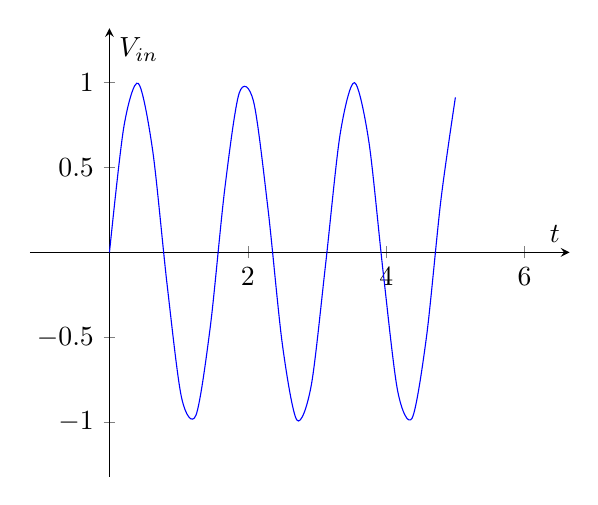
\begin{tikzpicture}
    \begin{axis}[
        domain=0:5,
        axis lines = middle,
        xmin = -0.5,
        xmax = 6,
        ymin = -1.1,
        ymax = 1.1,
        xlabel = $t$,
        ylabel = $V_{in}$,
        enlargelimits = true,
    ]
        \addplot[smooth,mark=none,color=blue] {sin(4*deg(x))};
    \end{axis}
\end{tikzpicture}
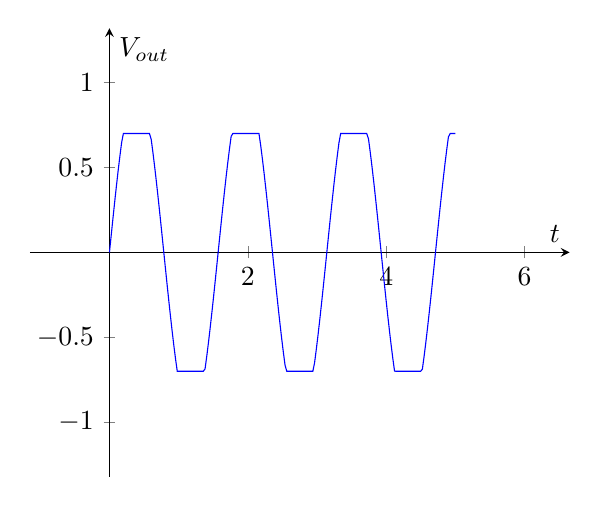
\begin{tikzpicture}
    \begin{axis}[
        domain=0:5,
        axis lines = middle,
        xmin = -0.5,
        xmax = 6,
        ymin = -1.1,
        ymax = 1.1,
        xlabel = $t$,
        ylabel = $V_{out}$,
        enlargelimits = true,
        y filter/.expression={y > 0.7 ? 0.7 : (y < -0.7 ? -0.7 : y)},
    ]
        \addplot[samples=200,mark=none,color=blue] {sin(4*deg(x))};
    \end{axis}
\end{tikzpicture}

  \caption{Impact of the diode limiter on the input sinusoidal voltage. Values that exceed the \SIrange{-0.7}{0.7}{V} range are clamped and the signal is distorted.}
  \label{fig:diode_limiter_signal}
\end{figure}


%%%%%%%%%%%%%%%%%%%%%%%%%%%%%%%%%%%%%%%%%%%%%%%%%%%%%%%%%%%%%%%%%%%%%%%%%%%%%%%%%%%%%%%
\subsection{First-Order Diode Clipper}
%%%%%%%%%%%%%%%%%%%%%%%%%%%%%%%%%%%%%%%%%%%%%%%%%%%%%%%%%%%%%%%%%%%%%%%%%%%%%%%%%%%%%%%
Combining the RC lowpass filter (\Figure{fig:rc_lowpass}) and the diode limiter (\Figure{fig:diode_limiter}) yields the first-order diode clipper (\Figure{fig:diode_clipper_circuit}). It is called "first-order" because only a single capacitor is used \cite{Parker2019}. If the input voltage is within the limiter's operational range, the circuit acts as a lowpass filter. If the voltage exceeds this range, it is clipped at the output and distortion is introduced.

The first-order diode clipper can be described by a nonlinear \ac{ODE} \cite{Yeh2007}
\begin{equation}
  \frac{\mathrm{d} V_\text{out}}{\mathrm{d}t} = \frac{V_\text{in} - V_\text{out}}{RC} - 2 \frac{I_\text{s}}{C} \sinh \left(\frac{V_\text{out}}{V_\text{t}}\right),
  \label{eq:diode_clipper_equation}
\end{equation}
where $V_\text{in}$ is the input voltage, $V_\text{out}$ is the output voltage, $t$ denotes time, $R$ is the serial resistance, $C$ is the parallel capacity, $I_\text{s}$ is the reverse saturation current, and $V_\text{t}$ is the thermal voltage. The last two are parameters of the diodes that can be measured \cite{Yeh2007}.

The parameter values of discrete elements used in the experiments were taken from \cite{Yeh2008}. They are summarized in \Table{tab:diode_clipper_element_parameters}.

\begin{table}
  \centering
  \caption{Parameter values of the discrete elements used in the diode clipper circuit. Source: \cite{Yeh2008}.}
  \begin{tabular}{c|c}
    \toprule
    \textbf{Parameter} & \textbf{Value} \\
    \midrule
    $R$ & \SI{2.2}{k\ohm} \\
    $C$ & \SI{10}{nF} \\
    $I_\text{s}$ & \SI{2.52}{nA} \\
    $V_\text{t}$ & \SI{45.3}{mV} \\
    \hline
  \end{tabular}
  \label{tab:diode_clipper_element_parameters}
\end{table}

$V_\text{in}$ is typically on the order of volts.

%%%%%%%%%%%%%%%%%%%%%%%%%%%%%%%%%%%%%%%%%%%%%%%%%%%%%%%%%%%%%%%%%%%%%%%%%%%%%%%%%%%%%%%
\subsection{Relation to Other Work}
%%%%%%%%%%%%%%%%%%%%%%%%%%%%%%%%%%%%%%%%%%%%%%%%%%%%%%%%%%%%%%%%%%%%%%%%%%%%%%%%%%%%%%%

The first-order diode clipper is a system particularly interesting in the context of ODENet, because it is governed by a known \ac{ODE} \cite{Yeh2007,Yeh2008}. Additionally, it was already modeled using a \ac{ResNet}-like architecture in \cite{Parker2019}. Thus, learning to imitate the diode clipper allowed the validation of ODENet and comparison to 
\begin{itemize}
    \item an \ac{LSTM}-based architecture from \cite{Wrightetal2020},
    \item a \ac{ResNet}-like architecture from \cite{Parker2019}, and
    \item a numerical solution using the \ac{ODE} from \cite{Yeh2007,Yeh2008}.
\end{itemize}

  \caption{Diode clipper circuit.}
  \label{fig:diode_clipper_circuit}
\end{figure}

The first-order diode clipper is a circuit frequently used to achieve signal distortion, e.g., in guitar amplifiers. Its schematic is shown in \Figure{fig:diode_clipper_circuit}. It can be regarded as consisting of two parts: an RC lowpass filter and a diode limiter.

Voltages and currents in this section are dependent on time, i.e., $V = V(t), I= I(t)$. For readability, this dependence is not stated explicitly in the equations.

%%%%%%%%%%%%%%%%%%%%%%%%%%%%%%%%%%%%%%%%%%%%%%%%%%%%%%%%%%%%%%%%%%%%%%%%%%%%%%%%%%%%%%%
\subsection{RC Lowpass Filter}
%%%%%%%%%%%%%%%%%%%%%%%%%%%%%%%%%%%%%%%%%%%%%%%%%%%%%%%%%%%%%%%%%%%%%%%%%%%%%%%%%%%%%%%

\begin{figure}
  \centering
  \begin{tikzpicture}
%--------start graphics code --------
% \draw[step=0.5,very thin, black!20] (-1,-0.5) grid (6,2.5);
\path (0,0) coordinate (ref_gnd);
\draw
  (ref_gnd)++(0,2) node[ocirc] {}
  node[xshift=-2mm,yshift=4mm] {$V_{in}$}
  to [R=\(R\)] ++(2,0) node[circ] {}
  to ++(1,0)  node[ocirc] {}
  node[yshift=4mm] {$V_{out}$}
  ++(-1,0)
  to [C=\(C\)] ++(0,-2)
  node[ground] {};
%--------end graphics code ----------
\end{tikzpicture}

  \caption{RC lowpass filter.}
  \label{fig:rc_lowpass}
\end{figure}

The first part of the diode clipper circuit is an RC lowpass filter. An RC lowpass filter is shown in \Figure{fig:rc_lowpass}. Given that the input voltage $V_\text{in}$ is a sine wave at frequency $f$, the input-output voltage relation is governed by the following equation
\begin{equation}
  V_\text{out} = \frac{X_C}{\sqrt{R^2 + X_C^2}} V_\text{in},
  \label{eq:rc_circuit}
\end{equation}
where $V_\text{out}$ is the output voltage, $X_C=\frac{1}{2\pi f C}$ is the capacitive reactance of the capacitor in the circuit, $C$ is its capacitance, and $R$ is the resistor's resistance.

The capacitor impedes low frequencies more; the lower the frequency, the higher the capacitive reactance. More capacitive reactance means larger voltage drop on the capacitor. Thus, assuming a constant magnitude across all frequencies of the input voltage, the output voltage is higher for low frequencies. Therefore, the circuit behaves like a lowpass filter.

Considering an arbitrary input waveform, we may derive a differential equation that describes the circuit \cite{Horowitz2015}. The current $I$ through the capacitor is proportional to the rate of change of the voltage across it

\begin{equation}
  I = C \frac{\mathrm{d}V_\text{out}}{\mathrm{d} t}.
  \label{eq:current_through_capacitor}
\end{equation}

The current flowing through the resistor can be calculated using the Ohm's law as a ratio of the voltage drop across the resistor to its resistance

\begin{equation}
  I = \frac{V_\text{in} - V_\text{out}}{R}.
  \label{eq:current_through_resistor}
\end{equation}

Because the same current flows through the resistor and the capacitor we can equate the right-hand sides of \Equation{eq:current_through_capacitor} and \Equation{eq:current_through_resistor}. After dividing by $C$, we obtain the final form of the \ac{ODE} describing the RC circuit

\begin{equation}
  \frac{\mathrm{d}V_\text{out}}{\mathrm{d} t} = \frac{V_\text{in} - V_\text{out}}{RC}.
\end{equation}



%%%%%%%%%%%%%%%%%%%%%%%%%%%%%%%%%%%%%%%%%%%%%%%%%%%%%%%%%%%%%%%%%%%%%%%%%%%%%%%%%%%%%%%
\subsection{Diode Limiter}
%%%%%%%%%%%%%%%%%%%%%%%%%%%%%%%%%%%%%%%%%%%%%%%%%%%%%%%%%%%%%%%%%%%%%%%%%%%%%%%%%%%%%%%
\begin{figure}
  \centering
  \begin{tikzpicture}
%--------start graphics code --------
% \draw[step=0.5,very thin, black!20] (-1,-0.5) grid (6,2.5);
\path (0,0) coordinate (ref_gnd);
\draw
  (ref_gnd)++(0,2) node[ocirc] {}
  node[xshift=-2mm,yshift=4mm] {$V_{in}$}
  to [R=\(R\)] ++(2,0) node[circ] {}
  to ++(2,0)  node[circ] {}
  to ++(1,0)  node[ocirc] {} {}
  node[yshift=4mm] {$V_{out}$}
  ++(-1,0)
  to [D] ++(0,-2)
  to ++(-1,0)
  node[ground] {}
  to ++(-1,0)
  to [D] ++(0,2);
%--------end graphics code ----------
\end{tikzpicture}

  \caption{Diode limiter circuit.}
  \label{fig:diode_limiter}
\end{figure}

The second part of the diode clipper is the diode limiter also called a \emph{diode clamp} \cite{Malvino2016}. Its circuit is shown in \Figure{fig:diode_limiter}. It consists of two inversely polarized diodes and a resistor. This circuit could be further divided into a \emph{positive clipper} (by removing the diode on the left) and a \emph{negative clipper} (by removing the diode on the right). These names refer to which part of the input \ac{AC} signal (the positive or the negative) is removed at the output.

If the diodes were ideal, i.e., they would behave as an open for voltages across smaller than 0 and as a short for voltages across larger than 0, $V_\text{out}$ would always be 0. However, to a second approximation, the diodes cause a voltage drop of \SI{0.7}{V} when conducting. Thus, the voltage cannot exceed the \SIrange{-0.7}{0.7}{V} range, being clamped when attempting to do so. The positive clipper guards the upper limit and the negative clipper guards the lower limit. The effect of passing an \ac{AC} signal through the diode limiter is shown in \Figure{fig:diode_limiter_signal}.

\cite{Yeh2007} contains a small-signal interpretation of the diode limiter circuit.

\begin{figure}
  \centering
  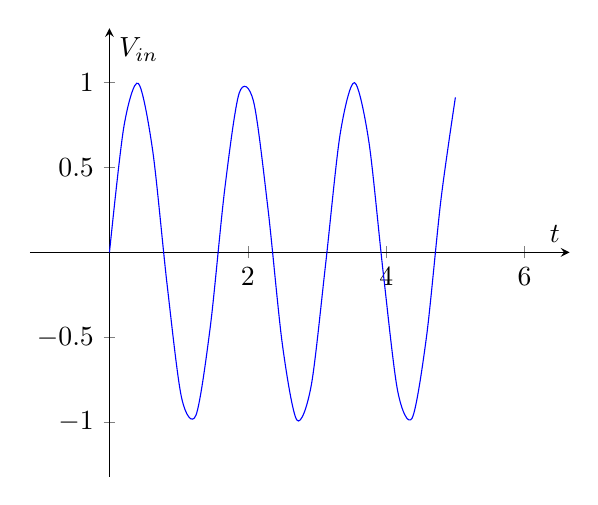
\begin{tikzpicture}
    \begin{axis}[
        domain=0:5,
        axis lines = middle,
        xmin = -0.5,
        xmax = 6,
        ymin = -1.1,
        ymax = 1.1,
        xlabel = $t$,
        ylabel = $V_{in}$,
        enlargelimits = true,
    ]
        \addplot[smooth,mark=none,color=blue] {sin(4*deg(x))};
    \end{axis}
\end{tikzpicture}
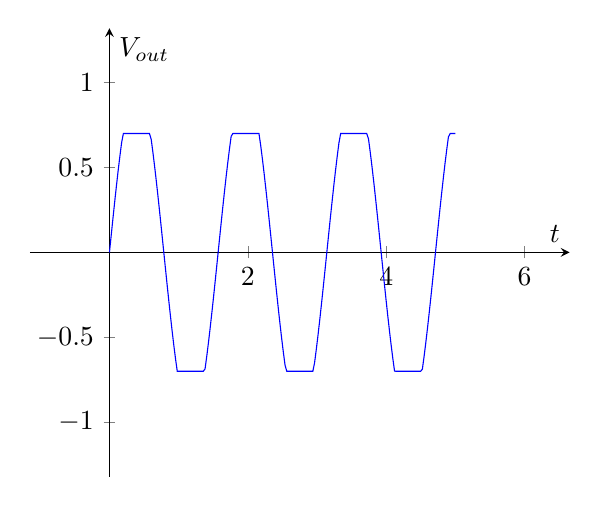
\begin{tikzpicture}
    \begin{axis}[
        domain=0:5,
        axis lines = middle,
        xmin = -0.5,
        xmax = 6,
        ymin = -1.1,
        ymax = 1.1,
        xlabel = $t$,
        ylabel = $V_{out}$,
        enlargelimits = true,
        y filter/.expression={y > 0.7 ? 0.7 : (y < -0.7 ? -0.7 : y)},
    ]
        \addplot[samples=200,mark=none,color=blue] {sin(4*deg(x))};
    \end{axis}
\end{tikzpicture}

  \caption{Impact of the diode limiter on the input sinusoidal voltage. Values that exceed the \SIrange{-0.7}{0.7}{V} range are clamped and the signal is distorted.}
  \label{fig:diode_limiter_signal}
\end{figure}


%%%%%%%%%%%%%%%%%%%%%%%%%%%%%%%%%%%%%%%%%%%%%%%%%%%%%%%%%%%%%%%%%%%%%%%%%%%%%%%%%%%%%%%
\subsection{First-Order Diode Clipper}
%%%%%%%%%%%%%%%%%%%%%%%%%%%%%%%%%%%%%%%%%%%%%%%%%%%%%%%%%%%%%%%%%%%%%%%%%%%%%%%%%%%%%%%
Combining the RC lowpass filter (\Figure{fig:rc_lowpass}) and the diode limiter (\Figure{fig:diode_limiter}) yields the first-order diode clipper (\Figure{fig:diode_clipper_circuit}). It is called "first-order" because only a single capacitor is used \cite{Parker2019}. If the input voltage is within the limiter's operational range, the circuit acts as a lowpass filter. If the voltage exceeds this range, it is clipped at the output and distortion is introduced.

The first-order diode clipper can be described by a nonlinear \ac{ODE} \cite{Yeh2007}
\begin{equation}
  \frac{\mathrm{d} V_\text{out}}{\mathrm{d}t} = \frac{V_\text{in} - V_\text{out}}{RC} - 2 \frac{I_\text{s}}{C} \sinh \left(\frac{V_\text{out}}{V_\text{t}}\right),
  \label{eq:diode_clipper_equation}
\end{equation}
where $V_\text{in}$ is the input voltage, $V_\text{out}$ is the output voltage, $t$ denotes time, $R$ is the serial resistance, $C$ is the parallel capacity, $I_\text{s}$ is the reverse saturation current, and $V_\text{t}$ is the thermal voltage. The last two are parameters of the diodes that can be measured \cite{Yeh2007}.

The parameter values of discrete elements used in the experiments were taken from \cite{Yeh2008}. They are summarized in \Table{tab:diode_clipper_element_parameters}.

\begin{table}
  \centering
  \caption{Parameter values of the discrete elements used in the diode clipper circuit. Source: \cite{Yeh2008}.}
  \begin{tabular}{c|c}
    \toprule
    \textbf{Parameter} & \textbf{Value} \\
    \midrule
    $R$ & \SI{2.2}{k\ohm} \\
    $C$ & \SI{10}{nF} \\
    $I_\text{s}$ & \SI{2.52}{nA} \\
    $V_\text{t}$ & \SI{45.3}{mV} \\
    \hline
  \end{tabular}
  \label{tab:diode_clipper_element_parameters}
\end{table}

$V_\text{in}$ is typically on the order of volts.

%%%%%%%%%%%%%%%%%%%%%%%%%%%%%%%%%%%%%%%%%%%%%%%%%%%%%%%%%%%%%%%%%%%%%%%%%%%%%%%%%%%%%%%
\subsection{Relation to Other Work}
%%%%%%%%%%%%%%%%%%%%%%%%%%%%%%%%%%%%%%%%%%%%%%%%%%%%%%%%%%%%%%%%%%%%%%%%%%%%%%%%%%%%%%%

The first-order diode clipper is a system particularly interesting in the context of ODENet, because it is governed by a known \ac{ODE} \cite{Yeh2007,Yeh2008}. Additionally, it was already modeled using a \ac{ResNet}-like architecture in \cite{Parker2019}. Thus, learning to imitate the diode clipper allowed the validation of ODENet and comparison to 
\begin{itemize}
    \item an \ac{LSTM}-based architecture from \cite{Wrightetal2020},
    \item a \ac{ResNet}-like architecture from \cite{Parker2019}, and
    \item a numerical solution using the \ac{ODE} from \cite{Yeh2007,Yeh2008}.
\end{itemize}

  \caption{Diode clipper circuit.}
  \label{fig:diode_clipper_circuit}
\end{figure}

The first-order diode clipper is a circuit frequently used to achieve signal distortion, e.g., in guitar amplifiers. Its schematic is shown in \Figure{fig:diode_clipper_circuit}. It can be regarded as consisting of two parts: an RC lowpass filter and a diode limiter.

Voltages and currents in this section are dependent on time, i.e., $V = V(t), I= I(t)$. For readability, this dependence is not stated explicitly in the equations.

%%%%%%%%%%%%%%%%%%%%%%%%%%%%%%%%%%%%%%%%%%%%%%%%%%%%%%%%%%%%%%%%%%%%%%%%%%%%%%%%%%%%%%%
\subsection{RC Lowpass Filter}
%%%%%%%%%%%%%%%%%%%%%%%%%%%%%%%%%%%%%%%%%%%%%%%%%%%%%%%%%%%%%%%%%%%%%%%%%%%%%%%%%%%%%%%

\begin{figure}
  \centering
  \begin{tikzpicture}
%--------start graphics code --------
% \draw[step=0.5,very thin, black!20] (-1,-0.5) grid (6,2.5);
\path (0,0) coordinate (ref_gnd);
\draw
  (ref_gnd)++(0,2) node[ocirc] {}
  node[xshift=-2mm,yshift=4mm] {$V_{in}$}
  to [R=\(R\)] ++(2,0) node[circ] {}
  to ++(1,0)  node[ocirc] {}
  node[yshift=4mm] {$V_{out}$}
  ++(-1,0)
  to [C=\(C\)] ++(0,-2)
  node[ground] {};
%--------end graphics code ----------
\end{tikzpicture}

  \caption{RC lowpass filter.}
  \label{fig:rc_lowpass}
\end{figure}

The first part of the diode clipper circuit is an RC lowpass filter. An RC lowpass filter is shown in \Figure{fig:rc_lowpass}. Given that the input voltage $V_\text{in}$ is a sine wave at frequency $f$, the input-output voltage relation is governed by the following equation
\begin{equation}
  V_\text{out} = \frac{X_C}{\sqrt{R^2 + X_C^2}} V_\text{in},
  \label{eq:rc_circuit}
\end{equation}
where $V_\text{out}$ is the output voltage, $X_C=\frac{1}{2\pi f C}$ is the capacitive reactance of the capacitor in the circuit, $C$ is its capacitance, and $R$ is the resistor's resistance.

The capacitor impedes low frequencies more; the lower the frequency, the higher the capacitive reactance. More capacitive reactance means larger voltage drop on the capacitor. Thus, assuming a constant magnitude across all frequencies of the input voltage, the output voltage is higher for low frequencies. Therefore, the circuit behaves like a lowpass filter.

Considering an arbitrary input waveform, we may derive a differential equation that describes the circuit \cite{Horowitz2015}. The current $I$ through the capacitor is proportional to the rate of change of the voltage across it

\begin{equation}
  I = C \frac{\mathrm{d}V_\text{out}}{\mathrm{d} t}.
  \label{eq:current_through_capacitor}
\end{equation}

The current flowing through the resistor can be calculated using the Ohm's law as a ratio of the voltage drop across the resistor to its resistance

\begin{equation}
  I = \frac{V_\text{in} - V_\text{out}}{R}.
  \label{eq:current_through_resistor}
\end{equation}

Because the same current flows through the resistor and the capacitor we can equate the right-hand sides of \Equation{eq:current_through_capacitor} and \Equation{eq:current_through_resistor}. After dividing by $C$, we obtain the final form of the \ac{ODE} describing the RC circuit

\begin{equation}
  \frac{\mathrm{d}V_\text{out}}{\mathrm{d} t} = \frac{V_\text{in} - V_\text{out}}{RC}.
\end{equation}



%%%%%%%%%%%%%%%%%%%%%%%%%%%%%%%%%%%%%%%%%%%%%%%%%%%%%%%%%%%%%%%%%%%%%%%%%%%%%%%%%%%%%%%
\subsection{Diode Limiter}
%%%%%%%%%%%%%%%%%%%%%%%%%%%%%%%%%%%%%%%%%%%%%%%%%%%%%%%%%%%%%%%%%%%%%%%%%%%%%%%%%%%%%%%
\begin{figure}
  \centering
  \begin{tikzpicture}
%--------start graphics code --------
% \draw[step=0.5,very thin, black!20] (-1,-0.5) grid (6,2.5);
\path (0,0) coordinate (ref_gnd);
\draw
  (ref_gnd)++(0,2) node[ocirc] {}
  node[xshift=-2mm,yshift=4mm] {$V_{in}$}
  to [R=\(R\)] ++(2,0) node[circ] {}
  to ++(2,0)  node[circ] {}
  to ++(1,0)  node[ocirc] {} {}
  node[yshift=4mm] {$V_{out}$}
  ++(-1,0)
  to [D] ++(0,-2)
  to ++(-1,0)
  node[ground] {}
  to ++(-1,0)
  to [D] ++(0,2);
%--------end graphics code ----------
\end{tikzpicture}

  \caption{Diode limiter circuit.}
  \label{fig:diode_limiter}
\end{figure}

The second part of the diode clipper is the diode limiter also called a \emph{diode clamp} \cite{Malvino2016}. Its circuit is shown in \Figure{fig:diode_limiter}. It consists of two inversely polarized diodes and a resistor. This circuit could be further divided into a \emph{positive clipper} (by removing the diode on the left) and a \emph{negative clipper} (by removing the diode on the right). These names refer to which part of the input \ac{AC} signal (the positive or the negative) is removed at the output.

If the diodes were ideal, i.e., they would behave as an open for voltages across smaller than 0 and as a short for voltages across larger than 0, $V_\text{out}$ would always be 0. However, to a second approximation, the diodes cause a voltage drop of \SI{0.7}{V} when conducting. Thus, the voltage cannot exceed the \SIrange{-0.7}{0.7}{V} range, being clamped when attempting to do so. The positive clipper guards the upper limit and the negative clipper guards the lower limit. The effect of passing an \ac{AC} signal through the diode limiter is shown in \Figure{fig:diode_limiter_signal}.

The analytical derivation of the differential equation governing the diode limiter circuit is more challenging than that of the first-order lowpass. Yeh et al. \cite{Yeh2007} present a small-signal interpretation of the diode limiter circuit.

\begin{figure}
  \centering
  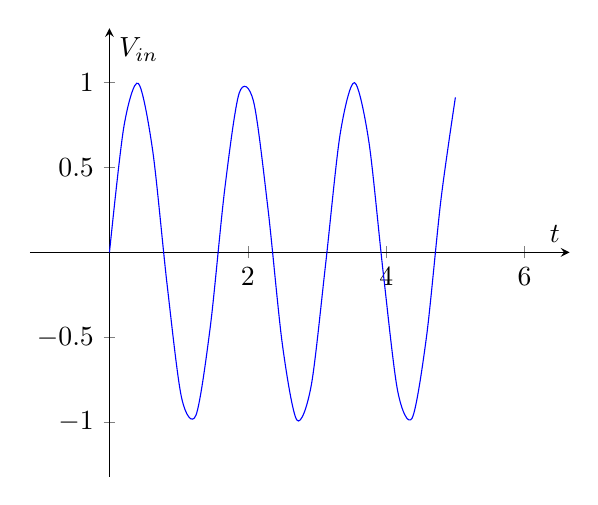
\begin{tikzpicture}
    \begin{axis}[
        domain=0:5,
        axis lines = middle,
        xmin = -0.5,
        xmax = 6,
        ymin = -1.1,
        ymax = 1.1,
        xlabel = $t$,
        ylabel = $V_{in}$,
        enlargelimits = true,
    ]
        \addplot[smooth,mark=none,color=blue] {sin(4*deg(x))};
    \end{axis}
\end{tikzpicture}
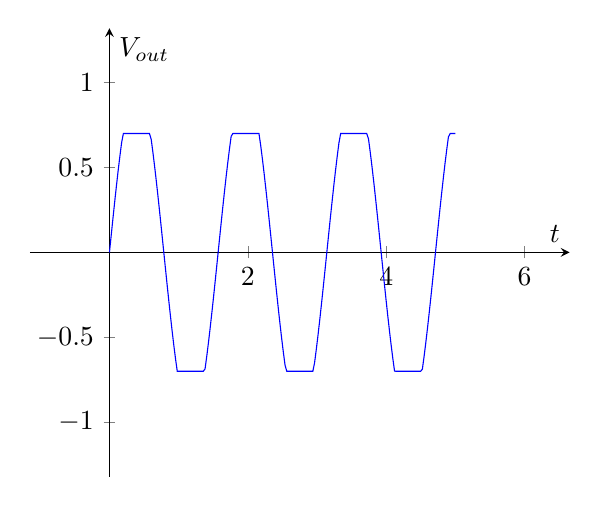
\begin{tikzpicture}
    \begin{axis}[
        domain=0:5,
        axis lines = middle,
        xmin = -0.5,
        xmax = 6,
        ymin = -1.1,
        ymax = 1.1,
        xlabel = $t$,
        ylabel = $V_{out}$,
        enlargelimits = true,
        y filter/.expression={y > 0.7 ? 0.7 : (y < -0.7 ? -0.7 : y)},
    ]
        \addplot[samples=200,mark=none,color=blue] {sin(4*deg(x))};
    \end{axis}
\end{tikzpicture}

  \caption{Impact of the diode limiter on the input sinusoidal voltage. Values that exceed the \SIrange{-0.7}{0.7}{V} range are clamped and the signal is distorted.}
  \label{fig:diode_limiter_signal}
\end{figure}


%%%%%%%%%%%%%%%%%%%%%%%%%%%%%%%%%%%%%%%%%%%%%%%%%%%%%%%%%%%%%%%%%%%%%%%%%%%%%%%%%%%%%%%
\subsection{First-Order Diode Clipper}
%%%%%%%%%%%%%%%%%%%%%%%%%%%%%%%%%%%%%%%%%%%%%%%%%%%%%%%%%%%%%%%%%%%%%%%%%%%%%%%%%%%%%%%
Combining the RC lowpass filter (\Figure{fig:rc_lowpass}) and the diode limiter (\Figure{fig:diode_limiter}) yields the first-order diode clipper (\Figure{fig:diode_clipper_circuit}). It is called "first-order" because only a single capacitor is used \cite{Parker2019}. If the input voltage is within the limiter's operational range, the circuit acts as a lowpass filter. If the voltage exceeds this range, it is clipped at the output and distortion is introduced.

The first-order diode clipper can be described by a nonlinear \ac{ODE} \cite{Yeh2007}
\begin{equation}
  \frac{\mathrm{d} V_\text{out}}{\mathrm{d}t} = \frac{V_\text{in} - V_\text{out}}{RC} - 2 \frac{I_\text{s}}{C} \sinh \left(\frac{V_\text{out}}{V_\text{t}}\right),
  \label{eq:diode_clipper_equation}
\end{equation}
where $V_\text{in}$ is the input voltage (typically on the order of volts), $V_\text{out}$ is the output voltage, $t$ denotes time, $R$ is the serial resistance, $C$ is the parallel capacity, $I_\text{s}$ is the reverse saturation current, and $V_\text{t}$ is the thermal voltage. The last two are parameters of the diodes that can be measured \cite{Yeh2007}.

The parameter values of discrete elements used in the experiments were taken from \cite{Yeh2008}. They are summarized in \Table{tab:diode_clipper_element_parameters}.

\begin{table}
  \centering
  \begin{tabular}{c|c}
    \toprule
    \textbf{Parameter} & \textbf{Value} \\
    \midrule
    $R$ & \SI{2.2}{k\ohm} \\
    $C$ & \SI{10}{nF} \\
    $I_\text{s}$ & \SI{2.52}{nA} \\
    $V_\text{t}$ & \SI{45.3}{mV} \\
    \hline
  \end{tabular}
  \caption{Parameter values of the discrete elements used in the diode clipper circuit. Source:~\cite{Yeh2008}.}
  \label{tab:diode_clipper_element_parameters}
\end{table}

%%%%%%%%%%%%%%%%%%%%%%%%%%%%%%%%%%%%%%%%%%%%%%%%%%%%%%%%%%%%%%%%%%%%%%%%%%%%%%%%%%%%%%%
\subsection{Relation to Other Work}
%%%%%%%%%%%%%%%%%%%%%%%%%%%%%%%%%%%%%%%%%%%%%%%%%%%%%%%%%%%%%%%%%%%%%%%%%%%%%%%%%%%%%%%

The first-order diode clipper is a system particularly interesting in the context of ODENet, because it is governed by a known \ac{ODE} \cite{Yeh2007,Yeh2008}. Additionally, it was already modeled using a \ac{ResNet}-like architecture in \cite{Parker2019}. Thus, learning to imitate the diode clipper allowed the validation of ODENet and comparison to 
\begin{itemize}
    \item an \ac{LSTM}-based architecture from \cite{Wrightetal2020},
    \item a \ac{ResNet}-like architecture from \cite{Parker2019}, and
    \item a numerical solution using the \ac{ODE} from \cite{Yeh2007,Yeh2008}.
\end{itemize}
